%!TEX root = ../main.tex
\chapter{Design}
In this section, I will discuss both aesthetic and technical designs for the application as well as offer a design of the system as a whole.

\section{System Design}
In order to gain a better overview of the system, I mapped out how the individual pieces of the system work together and analyzed each part.

\begin{figure}[ht]
	\centering
	\includegraphics[scale=0.55]{images/SystemDiagram.png}
	\caption{System Design Diagram}
	\label{fig:systemdesign}
\end{figure} 

\subsection{Server API}
In the initial stages of design, there were incorrect assumptions made about the project, which led to early diagrams being inaccurate and ultimately unworkable.
Initial designs attempted to implement all workflows into the applications and communicate directly between two phones, storing all necessary data/information on the client end. 
However, these designs presented many shortcomings. The main drawback was that communications between two mobile devices was unreliable, to the extent that it was not possible to ensure that data would remain synchronised between them.
For example, if a Child user marked a quest as completed, their phone would send a notification to the Parent user.
However, if this notification was not received by the Parent, the quest would fall into a limbo-like state where the Parent is waiting for it to be completed and the Child is waiting for it to be confirmed.

In order to prevent this type of occurrence, the system calls for a centralised location. This will allow two users to reliably communicate with each other.
By implementing the functionality into a server-based application, the system becomes significantly more portable. 
As all functionality of the system rests in a centralised location, any ported apps - such as iOS or a web app - would only have to tie into the existing Application Program Interface (API).
This would make porting the application simple, as the only code that would need to be created for these apps would be to simply send and receive web service requests to the API and display the data that it receives.

Setting up a central server has also meant increased maintainability of the software. 
Updating software on mobile phones/devices becomes difficult as people do not always update their apps to the latest version. 
Furthermore, if two users working together had different versions of the app it could cause serious interoperability problems.
The server API helps this, as all functionality updates to the system can be made in the server rather than user devices. This effectively distributes updated functionality to all users at once, instantly.

However, server-side implementation does have two main consequences that must be considered. 
Firstly, users would now require an internet connection to use the app so that it is able to communicate with the server.
This may cause difficulty for users who have limited data plans on their phone contracts or limited connectivity. 
However, this issue can be mitigated by keeping the data sent to a minimum and making the app only send absolutely necessary requests.
Furthermore, options exist in the Android operating system (OS) that restrict an application's data usage, meaning that requests will be halted until the user has connected to a usable wi-fi network.

Secondly, this would require all users to create an account with the server in order to use the app, as the system needs to store the data on the server end rather than on the users' phone.
I would need to have high security requirements surrounding that data, making sure that it is sufficiently encrypted during transit between the user device and server, and that the data stored on the server itself is sufficiently protected as well.

To handle logins securely, I plan on implementing a token-based authentication system within the server. 
Upon their first request, the user will submit their username and password within a HTTP POST request to the server.
The server then sends back an encrypted token that is derived out of various hashed attributes of their account, which the user client then stores.
The app will then authenticate itself with the server for every future request using this token.
This offers the main benefit that the app only has to store the token and not the username and password, which would leave it vulnerable to other (potentially malicious) apps accessing critical user data.
It will also mean that the app will not have to send the user's username and password with each request that it makes to the API, minimising the risk of the password being intercepted in transport.
The password is only stored within the server, which has securely encrypted it with a salted hash.

\subsection{Application}
The application will greet the user with a login/register screen that will be used to authenticate with the server before the rest of the app can be accessed.
The login process will be bypassed if the user currently has a valid authentication token.

The app will then communicate with the server to gather the relevant information needed for its current screen, being careful to only request what is necessary.
Once the information has been received, the app will display that information in a well-laid out manner and provide relevant options to add or update the data on the server.

On the first login of the app, the Child user will be prompted to enter a name for their character. 
They will then be instructed to pass the phone to the Parent who will create a PIN code.
Performing certain functions of the app will require this PIN code to be entered, thus preventing the Child from circumventing the nature of the app by giving themselves unlimited rewards.
Parents will be able to interact with the app solely through the Child's phone, but will also be able to set up an account on their own device which will provide the Parent functions remotely.
As a safety measure, this Parent account must be set up on the Child's device first, and will require the aforementioned PIN code to be activated/installed. 
This should ensure the Parent account belongs to an actual parent of that user, and cannot be misused by a malicious, unknown user. 

\subsection{Database}
\subsubsection{Design}
After planning out the requirements, the next step in the design of the project was to plan out the database structure.
I created an entity relationship diagram (ERD) to map out the various tables needed and the relationships between them.
ERDs are a useful visual representation of tables, columns and relationships within a database.
An ERD for the server application can be found in figure \ref{fig:erd}.
The requirements for the database are relatively simple: it is comprised of 3 tables and 26 data fields and will store all the necessary data about a user's account and their tasks.

\begin{figure}[ht]
	\centering
	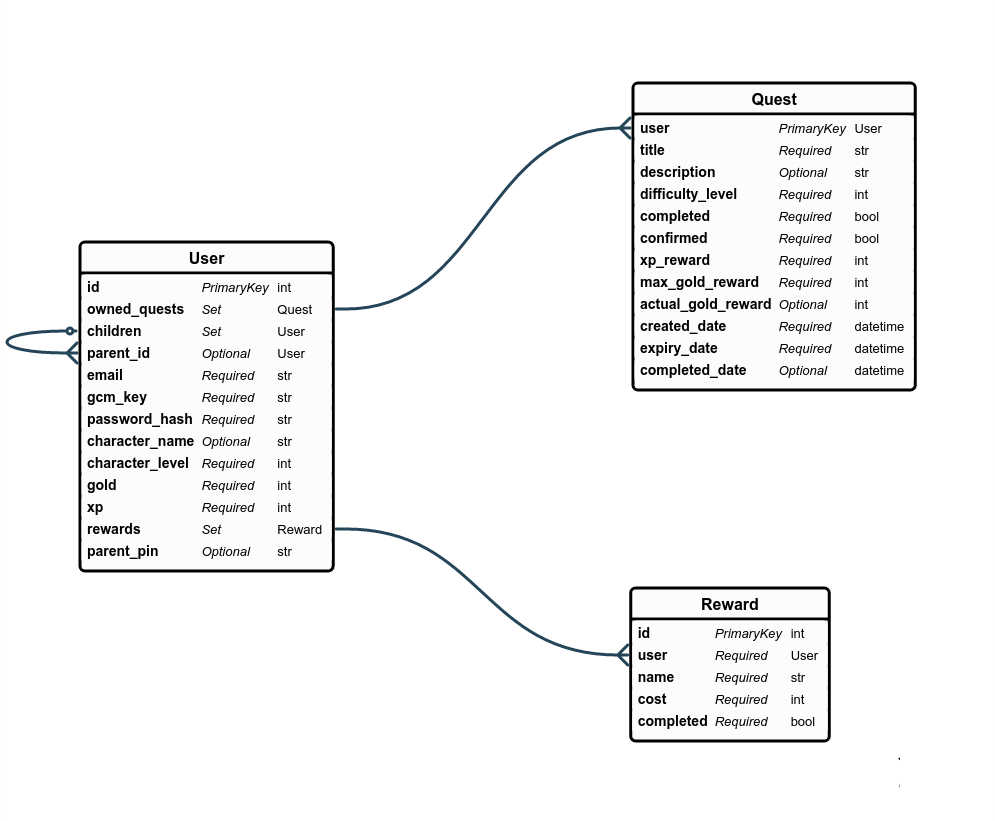
\includegraphics[scale=0.45]{../images/entityRelationshipDiagram.png}
	\caption{Server Entity Relationship Diagram}
	\label{fig:erd}
\end{figure}

\subsubsection{Database Access}
In this design, the central database is only accessible via the server API, rather than using a direct connection to any of the users' individual devices.
Instead, the server will offer publicly available web services that will provide functionality to input or update data. 
This has the benefit of allowing me to automatically validate and sanitise any data sent by the user before being added to the database and correctly reject requests that are unsuitable.
These services will ensure the user making the request is authorised to take actions on that account, i.e. the user making the request must be either the owner of that account or a registered Parent of the user - before allowing them to perform any functionality.
This segregation of the database helps to protect user data, as the database is not made accessible over the web at any point and is therefore less vulnerable to malicious entry.

\section{Chosen Methodology}
\cite{balaji2012waterfall} states that the choice of methodology depends on the project's requirements.
As raised in my risk analysis, there is a high risk of the project requirements changing as various assumptions about the project are challenged.
Therefore, influenced by the research in chapter 2, I have opted to develop the software artefact using an Agile methodology that would allow faster reaction to changes and issues that could otherwise put the project at risk.

\subsection{Test-Driven Development}
From the various development processes I have examined, I have chosen to use test-driven development (TDD), as it will be beneficial for the development of the server.
Due to the nature of how devices will communicate with the server, it will be simple to generate test cases from the various functions that the server offers.

As I have very little experience with TDD, it is likely that there will be a drop in developmental progress, as mentioned in the research in chapter two.
However, it must be considered that if the practice offers a higher quality of code, it is inherently likely to produce fewer errors and the productivity/time trade-off may be worth it.
However, due to the complexities of generating unit tests for Android, I have chosen to develop the application using only an Agile methodology.

\section{User Interface}
One of the components of software quality is usability and usefulness of it's User Interface (UI) \citep{isosoftwarequality}. 
As such, a focus must be put on making the screens of the application clearly usable.
The screens should not only be easy to use but easy to learn and navigate between. The interface should present minimal obstruction in the use of the application. 
The server application does not require an interface as its intended use is solely machine to machine communication.

\subsection{Screen Design}
\cite{stone2005user} classifies a good user interface design as an `easy, natural and engaging interaction between a user and a system'.

Wireframing is a useful tool to plan out the aesthetic design of screens and the UI elements used within them.
A wireframe is also useful to gain a clear overview of the navigation between screens, as they can be used to plan out the button presses that will select the next screen.
The wireframes shown in appendix \ref{appendix:wireframes} give an overview of the general aesthetic style that will be used.

\subsubsection{Your Quests Screen}
This will be a simple screen that displays the quests and potential rewards in an easy to read list.
The screen also offers a button used to mark a quest as complete, which will send this information to the Parent user for confirmation before rewards are offered.

\subsubsection{Character Screen}
This screen offers a quick overview of the user's character, gold, XP and the requirements needed to level up.
This will be the first screen that a Child user sees after logging in.

\subsubsection{Navigation Menu}
A navigation menu is necessary for the user to be able to change between screens with ease.
The menu will be customised to the type of user - Parent or Child - and certain options will require a Parent PIN code to gain access. 

\subsubsection{Add Quest Form}
This will be a simple screen for a Parent to input the necessary data about a quest and submit it to the server. 
The form only requires four inputs: A title for the quest; an optional longer description containing extra information; an estimated difficulty level of the task; and an expiry date.
I have opted to use a difficulty field that will tell the server what the XP/gold rewards should be, rather than having Parents manually input the rewards.
This is due to the fact that the Parent user is somewhat disconnected from the RPG elements of the application, and should see the app as more of a task management solution than a game.
I also believe that Parent users will find manually entering values of XP/gold tiresome and would find selecting a difficulty level easier. 

\subsection{Android Developer Guidelines}
\cite{materialdesignguidelines} have laid down clear guidelines on how to use the UI elements they have provided in the Android Source Development Kit.
By using these guidelines, the application will be more portable, as its UI will be more scalable to the various sizes of devices that are available.% UI is User Interface?
Following these guidelines will also help make the application maintainable, as following standards is a useful way of ensuring that other developers will be able to better understand the design used in this artefact.